\documentclass[xcolor=table]{beamer}
\usepackage{fontspec}
\usepackage{natbib}
\usepackage{booktabs}
\usepackage{xltxtra} 

\usepackage{polyglossia} 
\usepackage[table]{xcolor}
\usepackage{color}

\usepackage{multicol}
\usepackage{graphicx}
\usepackage{float}
\usepackage{hyperref} 
\hypersetup{bookmarks=false,bookmarksnumbered,bookmarksopenlevel=5,bookmarksdepth=5,xetex,colorlinks=true,linkcolor=blue,citecolor=blue}
\usepackage[all]{hypcap}
\usepackage{memhfixc}
\usepackage{lscape}
\usepackage{tikz}
\usetikzlibrary{trees}


\newfontfamily\gender[Mapping=tex-text,Numbers=OldStyle,Ligatures=Common]{Times New Roman} 
\newfontfamily\phon[Mapping=tex-text,Ligatures=Common,Scale=MatchLowercase,FakeSlant=0.3]{Charis SIL} 
\newcommand{\ipa}[1]{{\phon #1}} %API tjs en italique
 

\newfontfamily\cn[Mapping=tex-text,Ligatures=Common,Scale=MatchUppercase]{SimSun}%pour le chinois
\newcommand{\zh}[1]{{\cn #1}}
\newcommand{\hauteur}{5}
\newcommand{\gauche}{-3}
\newcommand{\courte}{1}
\newcommand{\longue}{2}
\newcommand{\diffh}{0.15}
\newcommand{\valeury}{0}
\newcommand{\valeurx}{0}
\newcommand{\soeur}{3}
\newcommand{\couple}{3}
\newcommand{\male}{{\gender ♂}}
\newcommand{\female}{{\gender ♀}}
\XeTeXlinebreaklocale "zh" %使用中文换行
\XeTeXlinebreakskip = 0pt plus 1pt %


\begin{document} 
  \begin{frame} 

 
 \title{\zh{茶堡嘉绒藏族的亲属称谓系统}}
 \author{Guillaume Jacques\\ \zh{(向柏霖)}\\CNRS CRLAO}
 \maketitle
\end{frame}   
  \begin{frame} 
 \frametitle{\zh{苏丹类型}} 
  \begin{tikzpicture}
 \renewcommand{\valeurx}{\gauche-\soeur/2}
 \renewcommand{\valeury}{\hauteur}
   \node (A) at (\valeurx-\diffh,\valeury) {};
   \node (B) at (\valeurx+\soeur+\diffh,\valeury) {};
   \node (C) at (\valeurx+\soeur/2,\valeury) {};
   \node (A1) at (\valeurx,\valeury+\diffh) {};
   \node (B1) at (\valeurx+\soeur,\valeury+\diffh) {};
   \node (C1) at (\valeurx+\soeur/2,\valeury+\diffh) {};
 \renewcommand{\valeury}{\hauteur-\courte}
   \node (D) at (\valeurx,\valeury) {FZ \female{} };
   \node (E) at (\valeurx+\soeur/2,\valeury) {FB \male{} };
   \node (F) at (\valeurx+\soeur,\valeury) {F \male{}};

 \renewcommand{\valeury}{\hauteur}
 \renewcommand{\valeurx}{\gauche-\soeur/2+\soeur+\couple}
   \node (A2) at (\valeurx-\diffh,\valeury) {};
   \node (B2) at (\valeurx+\soeur+\diffh,\valeury) {};
   \node (C2) at (\valeurx+\soeur/2,\valeury) {};
   \node (A3) at (\valeurx,\valeury+\diffh) {};
   \node (B3) at (\valeurx+\soeur,\valeury+\diffh) {};
   \node (C3) at (\valeurx+\soeur/2,\valeury+\diffh) {};
 \renewcommand{\valeury}{\hauteur-\courte}
   \node (G) at (\valeurx,\valeury) {M \female{} };
   \node (H) at (\valeurx+\soeur/2,\valeury) {MZ \female{} };
   \node (I) at (\valeurx+\soeur,\valeury) {MB \male{}};
   
   
 \renewcommand{\valeurx}{\gauche-\soeur/2+\soeur}
   \node (FG) at (\valeurx+\couple/2,\valeury+\diffh) {};
 \renewcommand{\valeury}{\hauteur-\longue}
   \node (FG1) at (\valeurx+\couple/2,\valeury-\diffh) {};
\renewcommand{\valeurx}{\gauche}
   \node (FG2) at (\valeurx+\soeur/2-\diffh,\valeury) {};
   \node (FG3) at (\valeurx+\soeur+\soeur/2+\diffh,\valeury) {};
   \node (FG5) at (\valeurx+\soeur+\soeur/2,\valeury+\diffh) {};
   \node (FG6) at (\valeurx+\soeur,\valeury+\diffh) {};
   \node (FG7) at (\valeurx+\soeur/2,\valeury+\diffh) {};
    \renewcommand{\valeurx}{\gauche}
 \renewcommand{\valeury}{\hauteur-\longue-\courte}   

   \node (K) at (\valeurx+\soeur+\soeur/2,\valeury) {Z \female{} };  
   \node (L) at (\valeurx+\soeur,\valeury) {EGO };  
   \node (M) at (\valeurx+\soeur/2,\valeury) {B \male{} };  
   \node (N) at (\valeurx-\soeur/2,\valeury) {FZD };      
   \node (O) at (\gauche-\soeur/2+\soeur+\couple+\soeur,\valeury) {MBS \male{} };  
\renewcommand{\valeury}{\hauteur-\longue-\longue-\courte}
\tikzstyle{ligne1}=[-,very thick,>=latex]    
\tikzstyle{ligne2}=[->,dotted,very thick,>=latex]
\tikzstyle{ligne3}=[->,very thick,>=latex]
\draw[ligne1] (A)--(B);
\draw[ligne1] (A1)--(D);
\draw[ligne1] (B1)--(F);
\draw[ligne1] (C1)--(E);

\draw[ligne1] (A2)--(B2);
\draw[ligne1] (A3)--(G);
\draw[ligne1] (B3)--(I);
\draw[ligne1] (C3)--(H);

\draw[ligne1] (F)--(G);
\draw[ligne1] (FG)--(FG1);
\draw[ligne1] (FG2)--(FG3);
\draw[ligne1] (FG5)--(K);
\draw[ligne1] (FG6)--(L);
\draw[ligne1] (FG7)--(M);

\draw[ligne1] (D)--(N);
\draw[ligne1] (I)--(O);

\end{tikzpicture}
\end{frame}   

  \begin{frame} 
 \frametitle{\zh{夏威夷类型}} 
  \begin{tikzpicture}
 \renewcommand{\valeurx}{\gauche-\soeur/2}
 \renewcommand{\valeury}{\hauteur}
   \node (A) at (\valeurx-\diffh,\valeury) {};
   \node (B) at (\valeurx+\soeur+\diffh,\valeury) {};
   \node (C) at (\valeurx+\soeur/2,\valeury) {};
   \node (A1) at (\valeurx,\valeury+\diffh) {};
   \node (B1) at (\valeurx+\soeur,\valeury+\diffh) {};
   \node (C1) at (\valeurx+\soeur/2,\valeury+\diffh) {};
 \renewcommand{\valeury}{\hauteur-\courte}
   \node (D) at (\valeurx,\valeury) {\colorbox{green}{FZ} \female{} };
   \node (E) at (\valeurx+\soeur/2,\valeury) {\colorbox{cyan}{FB} \male{} };
   \node (F) at (\valeurx+\soeur,\valeury) {F \male{}};

 \renewcommand{\valeury}{\hauteur}
 \renewcommand{\valeurx}{\gauche-\soeur/2+\soeur+\couple}
   \node (A2) at (\valeurx-\diffh,\valeury) {};
   \node (B2) at (\valeurx+\soeur+\diffh,\valeury) {};
   \node (C2) at (\valeurx+\soeur/2,\valeury) {};
   \node (A3) at (\valeurx,\valeury+\diffh) {};
   \node (B3) at (\valeurx+\soeur,\valeury+\diffh) {};
   \node (C3) at (\valeurx+\soeur/2,\valeury+\diffh) {};
 \renewcommand{\valeury}{\hauteur-\courte}
   \node (G) at (\valeurx,\valeury) {M \female{} };
   \node (H) at (\valeurx+\soeur/2,\valeury) {\colorbox{green}{MZ} \female{} };
   \node (I) at (\valeurx+\soeur,\valeury) {\colorbox{cyan}{MB} \male{}};
   
   
 \renewcommand{\valeurx}{\gauche-\soeur/2+\soeur}
   \node (FG) at (\valeurx+\couple/2,\valeury+\diffh) {};
 \renewcommand{\valeury}{\hauteur-\longue}
   \node (FG1) at (\valeurx+\couple/2,\valeury-\diffh) {};
\renewcommand{\valeurx}{\gauche}
   \node (FG2) at (\valeurx+\soeur/2-\diffh,\valeury) {};
   \node (FG3) at (\valeurx+\soeur+\soeur/2+\diffh,\valeury) {};
   \node (FG5) at (\valeurx+\soeur+\soeur/2,\valeury+\diffh) {};
   \node (FG6) at (\valeurx+\soeur,\valeury+\diffh) {};
   \node (FG7) at (\valeurx+\soeur/2,\valeury+\diffh) {};
    \renewcommand{\valeurx}{\gauche}
 \renewcommand{\valeury}{\hauteur-\longue-\courte}   

   \node (K) at (\valeurx+\soeur+\soeur/2,\valeury) {Z \female{} };  
   \node (L) at (\valeurx+\soeur,\valeury) {EGO };  
   \node (M) at (\valeurx+\soeur/2,\valeury) {B \male{} };  
   \node (N) at (\valeurx-\soeur/2,\valeury) {FZD };      
   \node (O) at (\gauche-\soeur/2+\soeur+\couple+\soeur,\valeury) {MBS \male{} };  
\renewcommand{\valeury}{\hauteur-\longue-\longue-\courte}
\tikzstyle{ligne1}=[-,very thick,>=latex]    
\tikzstyle{ligne2}=[->,dotted,very thick,>=latex]
\tikzstyle{ligne3}=[->,very thick,>=latex]
\draw[ligne1] (A)--(B);
\draw[ligne1] (A1)--(D);
\draw[ligne1] (B1)--(F);
\draw[ligne1] (C1)--(E);

\draw[ligne1] (A2)--(B2);
\draw[ligne1] (A3)--(G);
\draw[ligne1] (B3)--(I);
\draw[ligne1] (C3)--(H);

\draw[ligne1] (F)--(G);
\draw[ligne1] (FG)--(FG1);
\draw[ligne1] (FG2)--(FG3);
\draw[ligne1] (FG5)--(K);
\draw[ligne1] (FG6)--(L);
\draw[ligne1] (FG7)--(M);

\draw[ligne1] (D)--(N);
\draw[ligne1] (I)--(O);

\end{tikzpicture}
\end{frame}   

  \begin{frame} 
 \frametitle{\zh{爱斯基摩类型}} 
  \begin{tikzpicture}
 \renewcommand{\valeurx}{\gauche-\soeur/2}
 \renewcommand{\valeury}{\hauteur}
   \node (A) at (\valeurx-\diffh,\valeury) {};
   \node (B) at (\valeurx+\soeur+\diffh,\valeury) {};
   \node (C) at (\valeurx+\soeur/2,\valeury) {};
   \node (A1) at (\valeurx,\valeury+\diffh) {};
   \node (B1) at (\valeurx+\soeur,\valeury+\diffh) {};
   \node (C1) at (\valeurx+\soeur/2,\valeury+\diffh) {};
 \renewcommand{\valeury}{\hauteur-\courte}
   \node (D) at (\valeurx,\valeury) {\colorbox{green}{FZ} \female{} };
   \node (E) at (\valeurx+\soeur/2,\valeury) {\colorbox{cyan}{FB} \male{} };
   \node (F) at (\valeurx+\soeur,\valeury) {\colorbox{cyan}{F} \male{}};

 \renewcommand{\valeury}{\hauteur}
 \renewcommand{\valeurx}{\gauche-\soeur/2+\soeur+\couple}
   \node (A2) at (\valeurx-\diffh,\valeury) {};
   \node (B2) at (\valeurx+\soeur+\diffh,\valeury) {};
   \node (C2) at (\valeurx+\soeur/2,\valeury) {};
   \node (A3) at (\valeurx,\valeury+\diffh) {};
   \node (B3) at (\valeurx+\soeur,\valeury+\diffh) {};
   \node (C3) at (\valeurx+\soeur/2,\valeury+\diffh) {};
 \renewcommand{\valeury}{\hauteur-\courte}
   \node (G) at (\valeurx,\valeury) {\colorbox{green}{M} \female{} };
   \node (H) at (\valeurx+\soeur/2,\valeury) {\colorbox{green}{MZ} \female{} };
   \node (I) at (\valeurx+\soeur,\valeury) {\colorbox{cyan}{MB} \male{}};
   
   
 \renewcommand{\valeurx}{\gauche-\soeur/2+\soeur}
   \node (FG) at (\valeurx+\couple/2,\valeury+\diffh) {};
 \renewcommand{\valeury}{\hauteur-\longue}
   \node (FG1) at (\valeurx+\couple/2,\valeury-\diffh) {};
\renewcommand{\valeurx}{\gauche}
   \node (FG2) at (\valeurx+\soeur/2-\diffh,\valeury) {};
   \node (FG3) at (\valeurx+\soeur+\soeur/2+\diffh,\valeury) {};
   \node (FG5) at (\valeurx+\soeur+\soeur/2,\valeury+\diffh) {};
   \node (FG6) at (\valeurx+\soeur,\valeury+\diffh) {};
   \node (FG7) at (\valeurx+\soeur/2,\valeury+\diffh) {};
    \renewcommand{\valeurx}{\gauche}
 \renewcommand{\valeury}{\hauteur-\longue-\courte}   

   \node (K) at (\valeurx+\soeur+\soeur/2,\valeury) {\colorbox{yellow}{Z} \female{} };  
   \node (L) at (\valeurx+\soeur,\valeury) {EGO };  
   \node (M) at (\valeurx+\soeur/2,\valeury) {\colorbox{red}{B} \male{} };  
   \node (N) at (\valeurx-\soeur/2,\valeury) {\colorbox{yellow}{FZD} };      
   \node (O) at (\gauche-\soeur/2+\soeur+\couple+\soeur,\valeury) {\colorbox{red}{MBS} \male{} };  
\renewcommand{\valeury}{\hauteur-\longue-\longue-\courte}
\tikzstyle{ligne1}=[-,very thick,>=latex]    
\tikzstyle{ligne2}=[->,dotted,very thick,>=latex]
\tikzstyle{ligne3}=[->,very thick,>=latex]
\draw[ligne1] (A)--(B);
\draw[ligne1] (A1)--(D);
\draw[ligne1] (B1)--(F);
\draw[ligne1] (C1)--(E);

\draw[ligne1] (A2)--(B2);
\draw[ligne1] (A3)--(G);
\draw[ligne1] (B3)--(I);
\draw[ligne1] (C3)--(H);

\draw[ligne1] (F)--(G);
\draw[ligne1] (FG)--(FG1);
\draw[ligne1] (FG2)--(FG3);
\draw[ligne1] (FG5)--(K);
\draw[ligne1] (FG6)--(L);
\draw[ligne1] (FG7)--(M);

\draw[ligne1] (D)--(N);
\draw[ligne1] (I)--(O);

\end{tikzpicture}
\end{frame}   

  \begin{frame} 
 \frametitle{\zh{易洛魁类型}} 
  \begin{tikzpicture}
 \renewcommand{\valeurx}{\gauche-\soeur/2}
 \renewcommand{\valeury}{\hauteur}
   \node (A) at (\valeurx-\diffh,\valeury) {};
   \node (B) at (\valeurx+\soeur+\diffh,\valeury) {};
   \node (C) at (\valeurx+\soeur/2,\valeury) {};
   \node (A1) at (\valeurx,\valeury+\diffh) {};
   \node (B1) at (\valeurx+\soeur,\valeury+\diffh) {};
   \node (C1) at (\valeurx+\soeur/2,\valeury+\diffh) {};
 \renewcommand{\valeury}{\hauteur-\courte}
   \node (D) at (\valeurx,\valeury) {FZ \female{} };
   \node (E) at (\valeurx+\soeur/2,\valeury) {\colorbox{cyan}{FB} \male{} };
   \node (F) at (\valeurx+\soeur,\valeury) {\colorbox{cyan}{F} \male{}};

 \renewcommand{\valeury}{\hauteur}
 \renewcommand{\valeurx}{\gauche-\soeur/2+\soeur+\couple}
   \node (A2) at (\valeurx-\diffh,\valeury) {};
   \node (B2) at (\valeurx+\soeur+\diffh,\valeury) {};
   \node (C2) at (\valeurx+\soeur/2,\valeury) {};
   \node (A3) at (\valeurx,\valeury+\diffh) {};
   \node (B3) at (\valeurx+\soeur,\valeury+\diffh) {};
   \node (C3) at (\valeurx+\soeur/2,\valeury+\diffh) {};
 \renewcommand{\valeury}{\hauteur-\courte}
   \node (G) at (\valeurx,\valeury) {\colorbox{green}{M} \female{} };
   \node (H) at (\valeurx+\soeur/2,\valeury) {\colorbox{green}{MZ} \female{} };
   \node (I) at (\valeurx+\soeur,\valeury) {MB \male{}};
   
   
 \renewcommand{\valeurx}{\gauche-\soeur/2+\soeur}
   \node (FG) at (\valeurx+\couple/2,\valeury+\diffh) {};
 \renewcommand{\valeury}{\hauteur-\longue}
   \node (FG1) at (\valeurx+\couple/2,\valeury-\diffh) {};
\renewcommand{\valeurx}{\gauche}
   \node (FG2) at (\valeurx+\soeur/2-\diffh,\valeury) {};
   \node (FG3) at (\valeurx+\soeur+\soeur/2+\diffh,\valeury) {};
   \node (FG5) at (\valeurx+\soeur+\soeur/2,\valeury+\diffh) {};
   \node (FG6) at (\valeurx+\soeur,\valeury+\diffh) {};
   \node (FG7) at (\valeurx+\soeur/2,\valeury+\diffh) {};
    \renewcommand{\valeurx}{\gauche}
 \renewcommand{\valeury}{\hauteur-\longue-\courte}   

   \node (K) at (\valeurx+\soeur+\soeur/2,\valeury) {Z \female{} };  
   \node (L) at (\valeurx+\soeur,\valeury) {EGO };  
   \node (M) at (\valeurx+\soeur/2,\valeury) {B \male{} };  
   \node (N) at (\valeurx-\soeur/2,\valeury) {FZD };      
   \node (O) at (\gauche-\soeur/2+\soeur+\couple+\soeur,\valeury) {MBS \male{} };  
\renewcommand{\valeury}{\hauteur-\longue-\longue-\courte}
\tikzstyle{ligne1}=[-,very thick,>=latex]    
\tikzstyle{ligne2}=[->,dotted,very thick,>=latex]
\tikzstyle{ligne3}=[->,very thick,>=latex]
\draw[ligne1] (A)--(B);
\draw[ligne1] (A1)--(D);
\draw[ligne1] (B1)--(F);
\draw[ligne1] (C1)--(E);

\draw[ligne1] (A2)--(B2);
\draw[ligne1] (A3)--(G);
\draw[ligne1] (B3)--(I);
\draw[ligne1] (C3)--(H);

\draw[ligne1] (F)--(G);
\draw[ligne1] (FG)--(FG1);
\draw[ligne1] (FG2)--(FG3);
\draw[ligne1] (FG5)--(K);
\draw[ligne1] (FG6)--(L);
\draw[ligne1] (FG7)--(M);

\draw[ligne1] (D)--(N);
\draw[ligne1] (I)--(O);

\end{tikzpicture}
\end{frame}   


  \begin{frame} 
 \frametitle{\zh{奥马哈类型}} 
  \begin{tikzpicture}
 \renewcommand{\valeurx}{\gauche-\soeur/2}
 \renewcommand{\valeury}{\hauteur}
   \node (A) at (\valeurx-\diffh,\valeury) {};
   \node (B) at (\valeurx+\soeur+\diffh,\valeury) {};
   \node (C) at (\valeurx+\soeur/2,\valeury) {};
   \node (A1) at (\valeurx,\valeury+\diffh) {};
   \node (B1) at (\valeurx+\soeur,\valeury+\diffh) {};
   \node (C1) at (\valeurx+\soeur/2,\valeury+\diffh) {};
 \renewcommand{\valeury}{\hauteur-\courte}
   \node (D) at (\valeurx,\valeury) {FZ \female{} };
   \node (E) at (\valeurx+\soeur/2,\valeury) {FB \male{} };
   \node (F) at (\valeurx+\soeur,\valeury) {F \male{}};

 \renewcommand{\valeury}{\hauteur}
 \renewcommand{\valeurx}{\gauche-\soeur/2+\soeur+\couple}
   \node (A2) at (\valeurx-\diffh,\valeury) {};
   \node (B2) at (\valeurx+\soeur+\diffh,\valeury) {};
   \node (C2) at (\valeurx+\soeur/2,\valeury) {};
   \node (A3) at (\valeurx,\valeury+\diffh) {};
   \node (B3) at (\valeurx+\soeur,\valeury+\diffh) {};
   \node (C3) at (\valeurx+\soeur/2,\valeury+\diffh) {};
 \renewcommand{\valeury}{\hauteur-\courte}
   \node (G) at (\valeurx,\valeury) {M \female{} };
   \node (H) at (\valeurx+\soeur/2,\valeury) {MZ \female{} };
   \node (I) at (\valeurx+\soeur,\valeury) {\colorbox{cyan}{MB} \male{}};
   
   
 \renewcommand{\valeurx}{\gauche-\soeur/2+\soeur}
   \node (FG) at (\valeurx+\couple/2,\valeury+\diffh) {};
 \renewcommand{\valeury}{\hauteur-\longue}
   \node (FG1) at (\valeurx+\couple/2,\valeury-\diffh) {};
\renewcommand{\valeurx}{\gauche}
   \node (FG2) at (\valeurx+\soeur/2-\diffh,\valeury) {};
   \node (FG3) at (\valeurx+\soeur+\soeur/2+\diffh,\valeury) {};
   \node (FG5) at (\valeurx+\soeur+\soeur/2,\valeury+\diffh) {};
   \node (FG6) at (\valeurx+\soeur,\valeury+\diffh) {};
   \node (FG7) at (\valeurx+\soeur/2,\valeury+\diffh) {};
    \renewcommand{\valeurx}{\gauche}
 \renewcommand{\valeury}{\hauteur-\longue-\courte}   

   \node (K) at (\valeurx+\soeur+\soeur/2,\valeury) {Z \female{} };  
   \node (L) at (\valeurx+\soeur,\valeury) {EGO };  
   \node (M) at (\valeurx+\soeur/2,\valeury) {B \male{} };  
   \node (N) at (\valeurx-\soeur/2,\valeury) {FZD };      
   \node (O) at (\gauche-\soeur/2+\soeur+\couple+\soeur,\valeury) {\colorbox{cyan}{MBS} \male{} };  
\renewcommand{\valeury}{\hauteur-\longue-\longue-\courte}
\tikzstyle{ligne1}=[-,very thick,>=latex]    
\tikzstyle{ligne2}=[->,dotted,very thick,>=latex]
\tikzstyle{ligne3}=[->,very thick,>=latex]
\draw[ligne1] (A)--(B);
\draw[ligne1] (A1)--(D);
\draw[ligne1] (B1)--(F);
\draw[ligne1] (C1)--(E);

\draw[ligne1] (A2)--(B2);
\draw[ligne1] (A3)--(G);
\draw[ligne1] (B3)--(I);
\draw[ligne1] (C3)--(H);

\draw[ligne1] (F)--(G);
\draw[ligne1] (FG)--(FG1);
\draw[ligne1] (FG2)--(FG3);
\draw[ligne1] (FG5)--(K);
\draw[ligne1] (FG6)--(L);
\draw[ligne1] (FG7)--(M);

\draw[ligne1] (D)--(N);
\draw[ligne1] (I)--(O);

\end{tikzpicture}
\end{frame}   

  \begin{frame} 
 \frametitle{\zh{乌鸦类型}} 
  \begin{tikzpicture}
 \renewcommand{\valeurx}{\gauche-\soeur/2}
 \renewcommand{\valeury}{\hauteur}
   \node (A) at (\valeurx-\diffh,\valeury) {};
   \node (B) at (\valeurx+\soeur+\diffh,\valeury) {};
   \node (C) at (\valeurx+\soeur/2,\valeury) {};
   \node (A1) at (\valeurx,\valeury+\diffh) {};
   \node (B1) at (\valeurx+\soeur,\valeury+\diffh) {};
   \node (C1) at (\valeurx+\soeur/2,\valeury+\diffh) {};
 \renewcommand{\valeury}{\hauteur-\courte}
   \node (D) at (\valeurx,\valeury) {\colorbox{green}{FZ} \female{} };
   \node (E) at (\valeurx+\soeur/2,\valeury) {FB \male{} };
   \node (F) at (\valeurx+\soeur,\valeury) {F \male{}};

 \renewcommand{\valeury}{\hauteur}
 \renewcommand{\valeurx}{\gauche-\soeur/2+\soeur+\couple}
   \node (A2) at (\valeurx-\diffh,\valeury) {};
   \node (B2) at (\valeurx+\soeur+\diffh,\valeury) {};
   \node (C2) at (\valeurx+\soeur/2,\valeury) {};
   \node (A3) at (\valeurx,\valeury+\diffh) {};
   \node (B3) at (\valeurx+\soeur,\valeury+\diffh) {};
   \node (C3) at (\valeurx+\soeur/2,\valeury+\diffh) {};
 \renewcommand{\valeury}{\hauteur-\courte}
   \node (G) at (\valeurx,\valeury) {M \female{} };
   \node (H) at (\valeurx+\soeur/2,\valeury) {MZ \female{} };
   \node (I) at (\valeurx+\soeur,\valeury) {MB \male{}};
   
   
 \renewcommand{\valeurx}{\gauche-\soeur/2+\soeur}
   \node (FG) at (\valeurx+\couple/2,\valeury+\diffh) {};
 \renewcommand{\valeury}{\hauteur-\longue}
   \node (FG1) at (\valeurx+\couple/2,\valeury-\diffh) {};
\renewcommand{\valeurx}{\gauche}
   \node (FG2) at (\valeurx+\soeur/2-\diffh,\valeury) {};
   \node (FG3) at (\valeurx+\soeur+\soeur/2+\diffh,\valeury) {};
   \node (FG5) at (\valeurx+\soeur+\soeur/2,\valeury+\diffh) {};
   \node (FG6) at (\valeurx+\soeur,\valeury+\diffh) {};
   \node (FG7) at (\valeurx+\soeur/2,\valeury+\diffh) {};
    \renewcommand{\valeurx}{\gauche}
 \renewcommand{\valeury}{\hauteur-\longue-\courte}   

   \node (K) at (\valeurx+\soeur+\soeur/2,\valeury) {Z \female{} };  
   \node (L) at (\valeurx+\soeur,\valeury) {EGO };  
   \node (M) at (\valeurx+\soeur/2,\valeury) {B \male{} };  
   \node (N) at (\valeurx-\soeur/2,\valeury) {\colorbox{green}{FZD} };      
   \node (O) at (\gauche-\soeur/2+\soeur+\couple+\soeur,\valeury) {MBS \male{} };  
\renewcommand{\valeury}{\hauteur-\longue-\longue-\courte}
\tikzstyle{ligne1}=[-,very thick,>=latex]    
\tikzstyle{ligne2}=[->,dotted,very thick,>=latex]
\tikzstyle{ligne3}=[->,very thick,>=latex]
\draw[ligne1] (A)--(B);
\draw[ligne1] (A1)--(D);
\draw[ligne1] (B1)--(F);
\draw[ligne1] (C1)--(E);

\draw[ligne1] (A2)--(B2);
\draw[ligne1] (A3)--(G);
\draw[ligne1] (B3)--(I);
\draw[ligne1] (C3)--(H);

\draw[ligne1] (F)--(G);
\draw[ligne1] (FG)--(FG1);
\draw[ligne1] (FG2)--(FG3);
\draw[ligne1] (FG5)--(K);
\draw[ligne1] (FG6)--(L);
\draw[ligne1] (FG7)--(M);

\draw[ligne1] (D)--(N);
\draw[ligne1] (I)--(O);

\end{tikzpicture}
\end{frame}   

  \begin{frame} 
  
 \frametitle{\zh{嘉绒语研究}} 



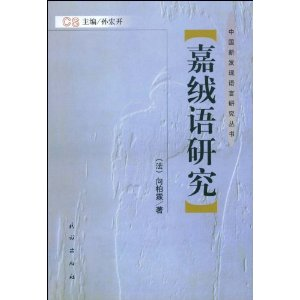
\includegraphics{fengmian.jpg}


\end{frame} 

  \begin{frame} 
  
 \frametitle{\zh{茶堡区嘉绒藏族}} 


  \begin{tikzpicture}
 \renewcommand{\valeurx}{\gauche-\soeur/2}
 \renewcommand{\valeury}{\hauteur}
   \node (A) at (\valeurx-\diffh,\valeury) {};
   \node (B) at (\valeurx+\soeur+\diffh,\valeury) {};
   \node (C) at (\valeurx+\soeur/2,\valeury) {};
   \node (A1) at (\valeurx,\valeury+\diffh) {};
   \node (B1) at (\valeurx+\soeur,\valeury+\diffh) {};
   \node (C1) at (\valeurx+\soeur/2,\valeury+\diffh) {};
 \renewcommand{\valeury}{\hauteur-\courte}
   \node (D) at (\valeurx,\valeury) {\ipa{tɤ-ɲi} \female{} };
   \node (E) at (\valeurx+\soeur/2,\valeury) {\ipa{tɤ-βɣo} \male{} };
   \node (F) at (\valeurx+\soeur,\valeury) {\ipa{tɤ-wa} \male{}};

 \renewcommand{\valeury}{\hauteur}
 \renewcommand{\valeurx}{\gauche-\soeur/2+\soeur+\couple}
   \node (A2) at (\valeurx-\diffh,\valeury) {};
   \node (B2) at (\valeurx+\soeur+\diffh,\valeury) {};
   \node (C2) at (\valeurx+\soeur/2,\valeury) {};
   \node (A3) at (\valeurx,\valeury+\diffh) {};
   \node (B3) at (\valeurx+\soeur,\valeury+\diffh) {};
   \node (C3) at (\valeurx+\soeur/2,\valeury+\diffh) {};
 \renewcommand{\valeury}{\hauteur-\courte}
   \node (G) at (\valeurx,\valeury) {\ipa{tɤ-mu} \female{} };
   \node (H) at (\valeurx+\soeur/2,\valeury) {\ipa{tɤ-laʁ} \female{} };
   \node (I) at (\valeurx+\soeur,\valeury) {\ipa{tɤ-rpɯ} \male{}};
   
   
 \renewcommand{\valeurx}{\gauche-\soeur/2+\soeur}
   \node (FG) at (\valeurx+\couple/2,\valeury+\diffh) {};
 \renewcommand{\valeury}{\hauteur-\longue}
   \node (FG1) at (\valeurx+\couple/2,\valeury-\diffh) {};
\renewcommand{\valeurx}{\gauche}
   \node (FG2) at (\valeurx-\diffh,\valeury) {};
   \node (FG3) at (\valeurx+\soeur+\soeur/2+\diffh,\valeury) {};
   \node (FG4) at (\valeurx,\valeury+\diffh) {};
   \node (FG5) at (\valeurx+\soeur+\soeur/2,\valeury+\diffh) {};
   \node (FG6) at (\valeurx+\soeur,\valeury+\diffh) {};
   \node (FG7) at (\valeurx+\soeur/2,\valeury+\diffh) {};
    \renewcommand{\valeurx}{\gauche}
 \renewcommand{\valeury}{\hauteur-\longue-\courte}   
   \node (J) at (\valeurx,\valeury) {\ipa{tɤ-pi } \female{}+ };  
   \node (K) at (\valeurx+\soeur+\soeur/2,\valeury) {\ipa{ta-ʁi } - };  
   \node (L) at (\valeurx+\soeur,\valeury) {EGO };  
   \node (M) at (\valeurx+\soeur/2,\valeury) {\ipa{tɤ-pi} \male{}+ };  
   \node (N) at (\valeurx-\soeur/2,\valeury) {\ipa{tɤ-ftsa}  };      
   \node (O) at (\gauche-\soeur/2+\soeur+\couple+\soeur,\valeury) {\ipa{tɤ-rpɯ} \male{} };  
\renewcommand{\valeury}{\hauteur-\longue-\longue-\courte}
   \node (P) at (\valeurx,\valeury) {\ipa{tɤ-ftsa}  };      
   \node (Q) at (\valeurx+\soeur/2,\valeury) {\ipa{tɤ-mdɯ}};      
\tikzstyle{ligne1}=[-,very thick,>=latex]    
\tikzstyle{ligne2}=[->,dotted,very thick,>=latex]
\tikzstyle{ligne3}=[->,very thick,>=latex]
\draw[ligne1] (A)--(B);
\draw[ligne1] (A1)--(D);
\draw[ligne1] (B1)--(F);
\draw[ligne1] (C1)--(E);

\draw[ligne1] (A2)--(B2);
\draw[ligne1] (A3)--(G);
\draw[ligne1] (B3)--(I);
\draw[ligne1] (C3)--(H);

\draw[ligne1] (F)--(G);
\draw[ligne1] (FG)--(FG1);
\draw[ligne1] (FG2)--(FG3);
\draw[ligne1] (FG4)--(J);
\draw[ligne1] (FG5)--(K);
\draw[ligne1] (FG6)--(L);
\draw[ligne1] (FG7)--(M);

\draw[ligne1] (D)--(N);
\draw[ligne1] (I)--(O);
\draw[ligne1] (J)--(P);
\draw[ligne1] (M)--(Q);
\end{tikzpicture}
%\end{figure}
\end{frame}



  \begin{frame} 
 \frametitle{\zh{茶堡区嘉绒藏族}} 


  \begin{tikzpicture}
 \renewcommand{\valeurx}{\gauche-\soeur/2}
 \renewcommand{\valeury}{\hauteur}
   \node (A) at (\valeurx-\diffh,\valeury) {};
   \node (B) at (\valeurx+\soeur+\diffh,\valeury) {};
   \node (C) at (\valeurx+\soeur/2,\valeury) {};
   \node (A1) at (\valeurx,\valeury+\diffh) {};
   \node (B1) at (\valeurx+\soeur,\valeury+\diffh) {};
   \node (C1) at (\valeurx+\soeur/2,\valeury+\diffh) {};
 \renewcommand{\valeury}{\hauteur-\courte}
   \node (D) at (\valeurx,\valeury) {\ipa{tɤ-ɲi} \female{} };
   \node (E) at (\valeurx+\soeur/2,\valeury) {\ipa{tɤ-βɣo} \male{} };
   \node (F) at (\valeurx+\soeur,\valeury) {\ipa{tɤ-wa} \male{}};

 \renewcommand{\valeury}{\hauteur}
 \renewcommand{\valeurx}{\gauche-\soeur/2+\soeur+\couple}
   \node (A2) at (\valeurx-\diffh,\valeury) {};
   \node (B2) at (\valeurx+\soeur+\diffh,\valeury) {};
   \node (C2) at (\valeurx+\soeur/2,\valeury) {};
   \node (A3) at (\valeurx,\valeury+\diffh) {};
   \node (B3) at (\valeurx+\soeur,\valeury+\diffh) {};
   \node (C3) at (\valeurx+\soeur/2,\valeury+\diffh) {};
 \renewcommand{\valeury}{\hauteur-\courte}
   \node (G) at (\valeurx,\valeury) {\ipa{tɤ-mu} \female{} };
   \node (H) at (\valeurx+\soeur/2,\valeury) {\ipa{tɤ-laʁ} \female{} };
   \node (I) at (\valeurx+\soeur,\valeury) {\colorbox{cyan}{\ipa{tɤ-rpɯ}} \male{}};
   
   
 \renewcommand{\valeurx}{\gauche-\soeur/2+\soeur}
   \node (FG) at (\valeurx+\couple/2,\valeury+\diffh) {};
 \renewcommand{\valeury}{\hauteur-\longue}
   \node (FG1) at (\valeurx+\couple/2,\valeury-\diffh) {};
\renewcommand{\valeurx}{\gauche}
   \node (FG2) at (\valeurx-\diffh,\valeury) {};
   \node (FG3) at (\valeurx+\soeur+\soeur/2+\diffh,\valeury) {};
   \node (FG4) at (\valeurx,\valeury+\diffh) {};
   \node (FG5) at (\valeurx+\soeur+\soeur/2,\valeury+\diffh) {};
   \node (FG6) at (\valeurx+\soeur,\valeury+\diffh) {};
   \node (FG7) at (\valeurx+\soeur/2,\valeury+\diffh) {};
    \renewcommand{\valeurx}{\gauche}
 \renewcommand{\valeury}{\hauteur-\longue-\courte}   
   \node (J) at (\valeurx,\valeury) {\ipa{tɤ-pi } \female{}+ };  
   \node (K) at (\valeurx+\soeur+\soeur/2,\valeury) {\ipa{ta-ʁi } - };  
   \node (L) at (\valeurx+\soeur,\valeury) {EGO };  
   \node (M) at (\valeurx+\soeur/2,\valeury) {\ipa{tɤ-pi} \male{}+ };  
   \node (N) at (\valeurx-\soeur/2,\valeury) {\ipa{tɤ-ftsa}  };      
   \node (O) at (\gauche-\soeur/2+\soeur+\couple+\soeur,\valeury) {\colorbox{cyan}{\ipa{tɤ-rpɯ}} \male{} };  
\renewcommand{\valeury}{\hauteur-\longue-\longue-\courte}
   \node (P) at (\valeurx,\valeury) {\ipa{tɤ-ftsa}  };      
   \node (Q) at (\valeurx+\soeur/2,\valeury) {\ipa{tɤ-mdɯ}};      
\tikzstyle{ligne1}=[-,very thick,>=latex]    
\tikzstyle{ligne2}=[->,dotted,very thick,>=latex]
\tikzstyle{ligne3}=[->,very thick,>=latex]
\draw[ligne1] (A)--(B);
\draw[ligne1] (A1)--(D);
\draw[ligne1] (B1)--(F);
\draw[ligne1] (C1)--(E);

\draw[ligne1] (A2)--(B2);
\draw[ligne1] (A3)--(G);
\draw[ligne1] (B3)--(I);
\draw[ligne1] (C3)--(H);

\draw[ligne1] (F)--(G);
\draw[ligne1] (FG)--(FG1);
\draw[ligne1] (FG2)--(FG3);
\draw[ligne1] (FG4)--(J);
\draw[ligne1] (FG5)--(K);
\draw[ligne1] (FG6)--(L);
\draw[ligne1] (FG7)--(M);

\draw[ligne1] (D)--(N);
\draw[ligne1] (I)--(O);
\draw[ligne1] (J)--(P);
\draw[ligne1] (M)--(Q);
\end{tikzpicture}
%\end{figure}
\end{frame}


  \begin{frame} 
 \frametitle{\zh{跨世代的称呼}} 


  \begin{tikzpicture}
 \renewcommand{\valeurx}{\gauche-\soeur/2}
 \renewcommand{\valeury}{\hauteur}
   \node (A) at (\valeurx-\diffh,\valeury) {};
   \node (B) at (\valeurx+\soeur+\diffh,\valeury) {};
   \node (C) at (\valeurx+\soeur/2,\valeury) {};
   \node (A1) at (\valeurx,\valeury+\diffh) {};
   \node (B1) at (\valeurx+\soeur,\valeury+\diffh) {};
   \node (C1) at (\valeurx+\soeur/2,\valeury+\diffh) {};
 \renewcommand{\valeury}{\hauteur-\courte}
   \node (D) at (\valeurx,\valeury) {\ipa{tɤ-ɲi} \female{} };
   \node (E) at (\valeurx+\soeur/2,\valeury) {\ipa{tɤ-βɣo} \male{} };
   \node (F) at (\valeurx+\soeur,\valeury) {\ipa{tɤ-wa} \male{}};

 \renewcommand{\valeury}{\hauteur}
 \renewcommand{\valeurx}{\gauche-\soeur/2+\soeur+\couple}
   \node (A2) at (\valeurx-\diffh,\valeury) {};
   \node (B2) at (\valeurx+\soeur+\diffh,\valeury) {};
   \node (C2) at (\valeurx+\soeur/2,\valeury) {};
   \node (A3) at (\valeurx,\valeury+\diffh) {};
   \node (B3) at (\valeurx+\soeur,\valeury+\diffh) {};
   \node (C3) at (\valeurx+\soeur/2,\valeury+\diffh) {};
 \renewcommand{\valeury}{\hauteur-\courte}
   \node (G) at (\valeurx,\valeury) {\ipa{tɤ-mu} \female{} };
   \node (H) at (\valeurx+\soeur/2,\valeury) {\ipa{tɤ-laʁ} \female{} };
   \node (I) at (\valeurx+\soeur,\valeury) {\colorbox{cyan}{\ipa{tɤ-rpɯ}} \male{}};
   
   
 \renewcommand{\valeurx}{\gauche-\soeur/2+\soeur}
   \node (FG) at (\valeurx+\couple/2,\valeury+\diffh) {};
 \renewcommand{\valeury}{\hauteur-\longue}
   \node (FG1) at (\valeurx+\couple/2,\valeury-\diffh) {};
\renewcommand{\valeurx}{\gauche}
   \node (FG2) at (\valeurx-\diffh,\valeury) {};
   \node (FG3) at (\valeurx+\soeur+\soeur/2+\diffh,\valeury) {};
   \node (FG4) at (\valeurx,\valeury+\diffh) {};
   \node (FG5) at (\valeurx+\soeur+\soeur/2,\valeury+\diffh) {};
   \node (FG6) at (\valeurx+\soeur,\valeury+\diffh) {};
   \node (FG7) at (\valeurx+\soeur/2,\valeury+\diffh) {};
    \renewcommand{\valeurx}{\gauche}
 \renewcommand{\valeury}{\hauteur-\longue-\courte}   
   \node (J) at (\valeurx,\valeury) {\ipa{tɤ-pi } \female{}+ };  
   \node (K) at (\valeurx+\soeur+\soeur/2,\valeury) {\ipa{ta-ʁi } - };  
   \node (L) at (\valeurx+\soeur,\valeury) {EGO };  
   \node (M) at (\valeurx+\soeur/2,\valeury) {\ipa{tɤ-pi} \male{}+ };  
   \node (N) at (\valeurx-\soeur/2,\valeury) {\colorbox{green}{\ipa{tɤ-ftsa}}  };      
   \node (O) at (\gauche-\soeur/2+\soeur+\couple+\soeur,\valeury) {\colorbox{cyan}{\ipa{tɤ-rpɯ}} \male{} };  
\renewcommand{\valeury}{\hauteur-\longue-\longue-\courte}
   \node (P) at (\valeurx,\valeury) {\colorbox{green}{\ipa{tɤ-ftsa}}  };      
   \node (Q) at (\valeurx+\soeur/2,\valeury) {\ipa{tɤ-mdɯ}};      
\tikzstyle{ligne1}=[-,very thick,>=latex]    
\tikzstyle{ligne2}=[->,dotted,very thick,>=latex]
\tikzstyle{ligne3}=[->,very thick,>=latex]
\draw[ligne1] (A)--(B);
\draw[ligne1] (A1)--(D);
\draw[ligne1] (B1)--(F);
\draw[ligne1] (C1)--(E);

\draw[ligne1] (A2)--(B2);
\draw[ligne1] (A3)--(G);
\draw[ligne1] (B3)--(I);
\draw[ligne1] (C3)--(H);

\draw[ligne1] (F)--(G);
\draw[ligne1] (FG)--(FG1);
\draw[ligne1] (FG2)--(FG3);
\draw[ligne1] (FG4)--(J);
\draw[ligne1] (FG5)--(K);
\draw[ligne1] (FG6)--(L);
\draw[ligne1] (FG7)--(M);

\draw[ligne1] (D)--(N);
\draw[ligne1] (I)--(O);
\draw[ligne1] (J)--(P);
\draw[ligne1] (M)--(Q);
\end{tikzpicture}
%\end{figure}
\end{frame}



  \begin{frame} 
 \frametitle{\zh{对兄弟姐妹的称呼(男性)}} 


  \begin{tikzpicture}
 \renewcommand{\valeurx}{\gauche-\soeur/2}
 \renewcommand{\valeury}{\hauteur}
   \node (A) at (\valeurx-\diffh,\valeury) {};
   \node (B) at (\valeurx+\soeur+\diffh,\valeury) {};
   \node (C) at (\valeurx+\soeur/2,\valeury) {};
   \node (A1) at (\valeurx,\valeury+\diffh) {};
   \node (B1) at (\valeurx+\soeur,\valeury+\diffh) {};
   \node (C1) at (\valeurx+\soeur/2,\valeury+\diffh) {};
 \renewcommand{\valeury}{\hauteur-\courte}
   \node (D) at (\valeurx,\valeury) {\ipa{tɤ-ɲi} \female{} };
   \node (E) at (\valeurx+\soeur/2,\valeury) {\ipa{tɤ-βɣo} \male{} };
   \node (F) at (\valeurx+\soeur,\valeury) {\ipa{tɤ-wa} \male{}};

 \renewcommand{\valeury}{\hauteur}
 \renewcommand{\valeurx}{\gauche-\soeur/2+\soeur+\couple}
   \node (A2) at (\valeurx-\diffh,\valeury) {};
   \node (B2) at (\valeurx+\soeur+\diffh,\valeury) {};
   \node (C2) at (\valeurx+\soeur/2,\valeury) {};
   \node (A3) at (\valeurx,\valeury+\diffh) {};
   \node (B3) at (\valeurx+\soeur,\valeury+\diffh) {};
   \node (C3) at (\valeurx+\soeur/2,\valeury+\diffh) {};
 \renewcommand{\valeury}{\hauteur-\courte}
   \node (G) at (\valeurx,\valeury) {\ipa{tɤ-mu} \female{} };
   \node (H) at (\valeurx+\soeur/2,\valeury) {\ipa{tɤ-laʁ} \female{} };
   \node (I) at (\valeurx+\soeur,\valeury) {\ipa{tɤ-rpɯ} \male{}};
   
   
 \renewcommand{\valeurx}{\gauche-\soeur/2+\soeur}
   \node (FG) at (\valeurx+\couple/2,\valeury+\diffh) {};
 \renewcommand{\valeury}{\hauteur-\longue}
   \node (FG1) at (\valeurx+\couple/2,\valeury-\diffh) {};
\renewcommand{\valeurx}{\gauche}
   \node (FG2) at (\valeurx+\soeur/2-\diffh,\valeury) {};
   \node (FG3) at (\valeurx+\soeur+\soeur/2+\diffh,\valeury) {};
   \node (FG5) at (\valeurx+\soeur+\soeur/2,\valeury+\diffh) {};
   \node (FG6) at (\valeurx+\soeur,\valeury+\diffh) {};
   \node (FG7) at (\valeurx+\soeur/2,\valeury+\diffh) {};
    \renewcommand{\valeurx}{\gauche}
 \renewcommand{\valeury}{\hauteur-\longue-\courte}   

   \node (K) at (\valeurx+\soeur+\soeur/2,\valeury) {\colorbox{green}{\ipa{tɤ-snom}} \female{} };  
   \node (L) at (\valeurx+\soeur,\valeury) {EGO };  
   \node (M) at (\valeurx+\soeur/2,\valeury) {\colorbox{green}{\ipa{tɤ-xtɤɣ}} \male{} };  
   \node (N) at (\valeurx-\soeur/2,\valeury) {\ipa{tɤ-ftsa}  };      
   \node (O) at (\gauche-\soeur/2+\soeur+\couple+\soeur,\valeury) {\ipa{tɤ-rpɯ} \male{} };  
\renewcommand{\valeury}{\hauteur-\longue-\longue-\courte}
\tikzstyle{ligne1}=[-,very thick,>=latex]    
\tikzstyle{ligne2}=[->,dotted,very thick,>=latex]
\tikzstyle{ligne3}=[->,very thick,>=latex]
\draw[ligne1] (A)--(B);
\draw[ligne1] (A1)--(D);
\draw[ligne1] (B1)--(F);
\draw[ligne1] (C1)--(E);

\draw[ligne1] (A2)--(B2);
\draw[ligne1] (A3)--(G);
\draw[ligne1] (B3)--(I);
\draw[ligne1] (C3)--(H);

\draw[ligne1] (F)--(G);
\draw[ligne1] (FG)--(FG1);
\draw[ligne1] (FG2)--(FG3);
\draw[ligne1] (FG5)--(K);
\draw[ligne1] (FG6)--(L);
\draw[ligne1] (FG7)--(M);

\draw[ligne1] (D)--(N);
\draw[ligne1] (I)--(O);

\end{tikzpicture}
%\end{figure}
\end{frame}

  \begin{frame} 
 \frametitle{\zh{对兄弟姐妹的称呼(女性)}} 


  \begin{tikzpicture}
 \renewcommand{\valeurx}{\gauche-\soeur/2}
 \renewcommand{\valeury}{\hauteur}
   \node (A) at (\valeurx-\diffh,\valeury) {};
   \node (B) at (\valeurx+\soeur+\diffh,\valeury) {};
   \node (C) at (\valeurx+\soeur/2,\valeury) {};
   \node (A1) at (\valeurx,\valeury+\diffh) {};
   \node (B1) at (\valeurx+\soeur,\valeury+\diffh) {};
   \node (C1) at (\valeurx+\soeur/2,\valeury+\diffh) {};
 \renewcommand{\valeury}{\hauteur-\courte}
   \node (D) at (\valeurx,\valeury) {\ipa{tɤ-ɲi} \female{} };
   \node (E) at (\valeurx+\soeur/2,\valeury) {\ipa{tɤ-βɣo} \male{} };
   \node (F) at (\valeurx+\soeur,\valeury) {\ipa{tɤ-wa} \male{}};

 \renewcommand{\valeury}{\hauteur}
 \renewcommand{\valeurx}{\gauche-\soeur/2+\soeur+\couple}
   \node (A2) at (\valeurx-\diffh,\valeury) {};
   \node (B2) at (\valeurx+\soeur+\diffh,\valeury) {};
   \node (C2) at (\valeurx+\soeur/2,\valeury) {};
   \node (A3) at (\valeurx,\valeury+\diffh) {};
   \node (B3) at (\valeurx+\soeur,\valeury+\diffh) {};
   \node (C3) at (\valeurx+\soeur/2,\valeury+\diffh) {};
 \renewcommand{\valeury}{\hauteur-\courte}
   \node (G) at (\valeurx,\valeury) {\ipa{tɤ-mu} \female{} };
   \node (H) at (\valeurx+\soeur/2,\valeury) {\ipa{tɤ-laʁ} \female{} };
   \node (I) at (\valeurx+\soeur,\valeury) {\ipa{tɤ-rpɯ} \male{}};
   
   
 \renewcommand{\valeurx}{\gauche-\soeur/2+\soeur}
   \node (FG) at (\valeurx+\couple/2,\valeury+\diffh) {};
 \renewcommand{\valeury}{\hauteur-\longue}
   \node (FG1) at (\valeurx+\couple/2,\valeury-\diffh) {};
\renewcommand{\valeurx}{\gauche}
   \node (FG2) at (\valeurx+\soeur/2-\diffh,\valeury) {};
   \node (FG3) at (\valeurx+\soeur+\soeur/2+\diffh,\valeury) {};
   \node (FG5) at (\valeurx+\soeur+\soeur/2,\valeury+\diffh) {};
   \node (FG6) at (\valeurx+\soeur,\valeury+\diffh) {};
   \node (FG7) at (\valeurx+\soeur/2,\valeury+\diffh) {};
    \renewcommand{\valeurx}{\gauche}
 \renewcommand{\valeury}{\hauteur-\longue-\courte}   

   \node (K) at (\valeurx+\soeur+\soeur/2,\valeury) {\colorbox{green}{\ipa{tɤ-sqhɤj}} \female{} };  
   \node (L) at (\valeurx+\soeur,\valeury) {EGO };  
   \node (M) at (\valeurx+\soeur/2,\valeury) {\colorbox{green}{\ipa{tɤ-wɤmɯ}} \male{} };  
   \node (N) at (\valeurx-\soeur/2,\valeury) {\ipa{tɤ-ftsa}  };      
   \node (O) at (\gauche-\soeur/2+\soeur+\couple+\soeur,\valeury) {\ipa{tɤ-rpɯ} \male{} };  
\renewcommand{\valeury}{\hauteur-\longue-\longue-\courte}
\tikzstyle{ligne1}=[-,very thick,>=latex]    
\tikzstyle{ligne2}=[->,dotted,very thick,>=latex]
\tikzstyle{ligne3}=[->,very thick,>=latex]
\draw[ligne1] (A)--(B);
\draw[ligne1] (A1)--(D);
\draw[ligne1] (B1)--(F);
\draw[ligne1] (C1)--(E);

\draw[ligne1] (A2)--(B2);
\draw[ligne1] (A3)--(G);
\draw[ligne1] (B3)--(I);
\draw[ligne1] (C3)--(H);

\draw[ligne1] (F)--(G);
\draw[ligne1] (FG)--(FG1);
\draw[ligne1] (FG2)--(FG3);
\draw[ligne1] (FG5)--(K);
\draw[ligne1] (FG6)--(L);
\draw[ligne1] (FG7)--(M);

\draw[ligne1] (D)--(N);
\draw[ligne1] (I)--(O);

\end{tikzpicture}

\end{frame}





%  \begin{frame} 
% \frametitle{\zh{茶堡区嘉绒藏族的亲属称谓系统}} 
%
%  \begin{tikzpicture}
% \renewcommand{\valeurx}{\gauche}
% \renewcommand{\valeury}{\hauteur}
%   \node (A) at (\valeurx-\diffh,\valeury) {};
%   \node (B) at (\valeurx+\soeur+\diffh,\valeury) {};
%   \node (C) at (\valeurx+\soeur/2,\valeury) {};
%   \node (A1) at (\valeurx,\valeury+\diffh) {};
%   \node (B1) at (\valeurx+\soeur,\valeury+\diffh) {};
% \renewcommand{\valeury}{\hauteur-\courte}
%   \node (C) at (\valeurx,\valeury) {\ipa{tɤ-rpɯ} ♂ };
%   \node (D) at (\valeurx+\soeur,\valeury) {\ipa{tɤ-ɬaʁ} ♀ };
%   \node (E) at (\valeurx+\couple,\valeury) {\ipa{tɤ-ɬaʁ} ♀};
%   \node (DE) at (\valeurx+\couple/2,\valeury+\diffh) {};
% \renewcommand{\valeury}{\hauteur-\longue}
%   \node (DE1) at (\valeurx+\couple/2,\valeury-\diffh) {};
%   \node (DE2) at (\valeurx-\diffh,\valeury) {};
%   \node (DE3) at (\valeurx+\soeur+\diffh,\valeury) {};
%   \node (DE4) at (\valeurx,\valeury+\diffh) {};
%   \node (DE5) at (\valeurx+\soeur,\valeury+\diffh) {};
% \renewcommand{\valeury}{\hauteur-\longue-\courte}   
%   \node (F) at (\valeurx,\valeury) {\ipa{tɤ-rpɯ} ♂ };  
%   \node (F1) at (\valeurx+\couple,\valeury) {\ipa{tɤ-ɬaʁ} ♀ };   
%   \node (G) at (\valeurx+\soeur,\valeury) {\ipa{tɤ-ɬaʁ} ♀ };  
%   \node (FG) at (\valeurx+\couple/2,\valeury+\diffh) {};
% \renewcommand{\valeury}{\hauteur-\longue-\longue}   
%   \node (FG1) at (\valeurx+\couple/2,\valeury-\diffh) {};
%   \node (FG2) at (\valeurx-\diffh,\valeury) {};
%   \node (FG3) at (\valeurx+\couple+\diffh,\valeury) {};
%   \node (FG4) at (\valeurx,\valeury+\diffh) {};
%   \node (FG5) at (\valeurx+\couple,\valeury+\diffh) {};
% \renewcommand{\valeury}{\hauteur-\longue-\longue-\courte}   
%   \node (H) at (\valeurx,\valeury) {\ipa{tɤ-rpɯ} ♂ };   
%   \node (I) at (\valeurx+\couple,\valeury) {\ipa{tɤ-ɬaʁ} ♀ };  
%   
%% 		\begin{tabular}[l] \Delta \\ 
%%   			\ipa{tɤ-rpɯ} %\\ \end{tabular}   
%   
%    
%\tikzstyle{ligne1}=[-,very thick,>=latex]    
%\tikzstyle{ligne2}=[->,dotted,very thick,>=latex]
%\tikzstyle{ligne3}=[->,very thick,>=latex]
%\draw[ligne1] (A)--(B);
%\draw[ligne1] (A1)--(C);
%\draw[ligne1] (B1)--(D);
%\draw[ligne1] (C)--(E);
%
%\draw[ligne1] (DE)--(DE1);
%\draw[ligne1] (DE2)--(DE3);
%\draw[ligne1] (DE4)--(F);
%\draw[ligne1] (DE5)--(G);
%
%\draw[ligne1] (F)--(F1);
%\draw[ligne1] (FG)--(FG1);
%\draw[ligne1] (FG2)--(FG3);
%\draw[ligne1] (FG4)--(H);
%\draw[ligne1] (FG5)--(I);
%
%\end{tikzpicture}
%\end{frame}


  \begin{frame} 
 \frametitle{\zh{茶堡话亲属称谓的形态变化}} 
 

\begin{tabular}{lllllllll} \toprule
 \zh{代词} & \zh{领属前缀} & \\
\midrule
 \ipa{aʑo},    \ipa{ɤj} &	\ipa{a-xtɤɣ}  &	 \zh{我的兄弟} \\
\ipa{nɤʑo},  \ipa{nɤj} &	\ipa{nɤ-xtɤɣ}  & \zh{你的兄弟} \\
\ipa{ɯʑo}  &	\ipa{ɯ-xtɤɣ}  &		 \zh{他的的兄弟} \\
\ipa{tɕiʑo}  &	\ipa{tɕi-xtɤɣ}  &	 \zh{我俩的的兄弟} \\
\ipa{ndʑiʑo}  &	\ipa{ndʑi-xtɤɣ}  &	 \zh{你俩的兄弟} \\	
\ipa{ʑɤni}  &	\ipa{ndʑi-xtɤɣ}  &	 \zh{他俩的的兄弟} \\	
\ipa{iʑo}, \ipa{iʑora}      &	\ipa{i-xtɤɣ}  &			 \zh{我们的兄弟} \\
\ipa{nɯʑo}, \ipa{nɯʑora},   \ipa{nɯʑɤra}  &	\ipa{nɯ-xtɤɣ}  &			 \zh{你们的兄弟} \\
\ipa{ʑara}  &	\ipa{nɯ-xtɤɣ}  &	 \zh{他们的兄弟} \\
   &	\ipa{tɤ-xtɤɣ}  &	 \zh{兄弟} \\
\bottomrule
\end{tabular}

\end{frame}

\end{document}
